\documentclass[twocolumn]{article}
\usepackage[utf8]{inputenc}
\usepackage{changepage}
\usepackage{graphicx}
\usepackage{amsmath}
\usepackage{amssymb}
\usepackage{amsthm}
\usepackage{mathtools}
\usepackage{float}
\usepackage[siunitx]{circuitikz}
\usepackage{tikz}
\usepackage{pgfplots}
\usepackage[colorlinks=true, linkcolor=black, citecolor=black, urlcolor=blue]{hyperref}
\usepackage{listings}
\pgfplotsset{width=10cm,compat=1.9}
\usetikzlibrary{positioning, arrows.meta}
\usepackage[a4paper, total={6in, 10in}]{geometry}
\usepackage{cite}
\bibliographystyle{ieeetr}

\title{\textbf{PROJECT VOICE - Continuous Decompositon Analysis and Signal Modeling For Galvanic Skin Response}}
\author{\textbf{Julian Edelman}}

\begin{document}

\maketitle

\section*{Introduction}

Galvanic Skin Response (GSR) measures the electrical conductance of the skin, which varies with its moisture level. This physiological signal is widely used in psychophysiological research to infer sympathetic nervous system activity, reflecting emotional and cognitive states. GSR signals comprise two primary components: the \emph{tonic} component, representing the slow-varying baseline skin conductance level, and the \emph{phasic} component, consisting of rapid fluctuations due to discrete stimuli or spontaneous neural activity.

Continuous Decomposition Analysis (CDA) is a method used to separate the tonic and phasic components of GSR signals. This document explains the mathematical concepts and processes involved in preprocessing GSR data and performing CDA using non-negative deconvolution.

\section*{Signal Modeling and Preprocessing}

The observed GSR signal \( y(t) \) can be modeled as the sum of the tonic component \( T(t) \), the phasic component \( P(t) \), and measurement noise \( n(t) \) \cite{Dawson2007,Boucsein2012,Braithwaite2013}:

\begin{equation}
y(t) = T(t) + P(t) + n(t).
\end{equation}

\subsection*{Tonic Component}

The tonic component \( T(t) \) represents the slow variations in skin conductance over time, often modeled as a low-frequency trend \cite{Dawson2007,Boucsein2012}:

\begin{equation}
T(t) = a + b t,
\end{equation}

where \( a \) is the baseline conductance, and \( b \) is the drift rate.

\subsection*{Phasic Component}

The phasic component \( P(t) \) consists of rapid, transient increases in skin conductance known as Skin Conductance Responses (SCRs). Each SCR can be modeled as an exponentially decaying function triggered at time \( t_i \) \cite{Dawson2007,Boucsein2012,Braithwaite2013}:

\begin{equation}
P(t) = \sum_{i} A_i e^{-\frac{(t - t_i)}{\tau}} u(t - t_i),
\end{equation}

where \( A_i \) is the amplitude of the \( i \)-th SCR, \( \tau \) is the decay time constant, and \( u(t) \) is the unit step function ensuring causality.

\subsection*{Preprocessing Steps}

To prepare the GSR signal for analysis, several preprocessing steps are performed. The preprocessing is done to clean the signal, making it easier to work with.

\subsubsection*{Low-Pass Filtering}

High-frequency noise is removed using a low-pass Butterworth filter. This will prevent aliasing when downsampling. The filter is designed with a cut-off frequency \( f_c \) and applied to the signal \( y(t) \).

\subsubsection*{Downsampling}

The signal is downsampled to reduce data size and focus on the frequency content of interest. If the original sampling frequency is \( f_s \) and the new sampling frequency is \( f_{\text{new}} \), the downsampling factor \( D \) is:

\begin{equation}
D = \frac{f_s}{f_{\text{new}}}.
\end{equation}

The signal is then downsampled by keeping every \( D \)-th sample.

Residual high-frequency noise is reduced using a moving average filter with window size \( M \). Let the preprocessed signal after downsampling be represented by \( y[n] \), where \( n \) is the discrete time index. The smoothed signal \( \tilde{y}[n] \) is calculated as:

\begin{equation}
\tilde{y}[n] = \frac{1}{M} \sum_{k=0}^{M-1} y[n - k].
\end{equation}

This equation computes the average of \( M \) consecutive samples, smoothing out rapid fluctuations due to noise.

\section*{Continuous Decomposition Analysis (CDA)}

The goal of CDA is to estimate the underlying neural driver function \( d(t) \) that generates the phasic component \( P(t) \) through convolution with an Impulse Response Function (IRF). The process involves defining the IRF, modeling the convolution, and performing deconvolution under non-negativity constraints.

\subsection*{Impulse Response Function (IRF)}

The IRF \( h(t) \) models the skin conductance response to a unit neural impulse. A biexponential function is commonly used \cite{nihDecompositionSkin}:

\begin{equation}
h(t) = \frac{1}{\tau_1 - \tau_2} \left( e^{-\frac{t}{\tau_1}} - e^{-\frac{t}{\tau_2}} \right) u(t),
\end{equation}

where \( \tau_1 \) is the rise time constant, \( \tau_2 \) is the decay time constant, and \( u(t) \) ensures causality. The IRF is normalized to have a maximum amplitude of 1:

\begin{equation}
h_{\text{normalized}}(t) = \frac{h(t)}{\max h(t)}.
\end{equation}

\subsection*{Convolution Model}

The phasic component \( P(t) \) is modeled as the convolution of the driver function \( d(t) \) with the IRF \( h(t) \):

\begin{equation}
P(t) = \int_{0}^{t} h(t - \tau) d(\tau) d\tau = (h * d)(t).
\end{equation}

\subsection*{Deconvolution Problem}

The observed signal \( y(t) \) is the sum of \( T(t) \) and \( P(t) \). The deconvolution aims to recover \( d(t) \) given \( y(t) \) and \( h(t) \). This can be formulated in discrete time as \cite{nihDecompositionSkin}:

\begin{equation}
\mathbf{y} = \mathbf{K} \mathbf{d} + \mathbf{T} + \mathbf{n},
\end{equation}

where:

\begin{itemize}
    \item \( \mathbf{y} \) is the vector of observed data.
    \item \( \mathbf{K} \) is the convolution matrix constructed from \( h(t) \).
    \item \( \mathbf{d} \) is the driver function vector.
    \item \( \mathbf{T} \) is the tonic component vector.
    \item \( \mathbf{n} \) is the noise vector.
\end{itemize}

Assuming \( \mathbf{T} \) varies slowly, it can be estimated or modeled separately.

\subsection*{Non-Negative Deconvolution}

As proposed by Benedek and Kaernbach \cite{nihDecompositionSkin}, the deconvolution is performed under the constraint that \( d(t) \geq 0 \) because neural activations cannot be negative. The optimization problem is:

\begin{equation}
\min_{\mathbf{d} \geq 0} \left\| \mathbf{K} \mathbf{d} - \mathbf{y} \right\|_2^2 + \lambda \left\| \mathbf{d} \right\|_2^2,
\end{equation}

where \( \lambda \) is a regularization parameter that balances data fidelity and smoothness.

\subsection*{Solution via Non-Negative Least Squares (NNLS)}

The optimization problem is solved using Non-Negative Least Squares (NNLS) methods \cite{article}:

\begin{equation}
\mathbf{d} = \arg\min_{\mathbf{d} \geq 0} \left( \left\| \mathbf{K} \mathbf{d} - \mathbf{y} \right\|_2^2 + \lambda \left\| \mathbf{d} \right\|_2^2 \right).
\end{equation}

The regularization term \( \lambda \left\| \mathbf{d} \right\|_2^2 \) penalizes large values of \( \mathbf{d} \) to prevent overfitting. Efficient numerical algorithms, such as the Lawson-Hanson algorithm, can be used to solve the NNLS problem while handling the non-negativity constraints.

\subsection*{Reconstruction of Components}

Once \( \mathbf{d} \) is estimated, the phasic component is reconstructed as \cite{nihDecompositionSkin}:

\begin{equation}
\mathbf{P} = \mathbf{K} \mathbf{d}.
\end{equation}

The tonic component is then obtained by subtracting the phasic component from the preprocessed signal:

\begin{equation}
\mathbf{T} = \mathbf{y} - \mathbf{P}.
\end{equation}

\section*{Interpretation of Results}

The estimated driver function \( \mathbf{d} \) reveals the timing and magnitude of neural activations that elicit SCRs. Peaks in \( \mathbf{d} \) correspond to significant sympathetic nervous system events. The reconstructed phasic component \( \mathbf{P} \) reflects the rapid changes in skin conductance due to these activations, while the tonic component \( \mathbf{T} \) represents the baseline conductance level.

By analyzing \( \mathbf{d} \), physiological responses to stimuli can be identified and quantified. The separation of tonic and phasic components allows for a more precise assessment of autonomic nervous system activity.

\section*{Analysis of Generated Signal and Resulting Graphs}

In this section, we analyze the generated synthetic GSR signal and interpret the resulting graphs produced by the program. The figures illustrate the various stages of signal processing and decomposition, providing insights into the characteristics of the GSR signal and the effectiveness of the Continuous Decomposition Analysis.

\section*{Analysis of Generated Signal and Resulting Graphs}

In this section, we analyze the generated synthetic GSR signal and interpret the resulting graphs produced by the program. The figures illustrate the various stages of signal processing and decomposition, providing insights into the characteristics of the GSR signal and the effectiveness of the Continuous Decomposition Analysis.

\subsection*{Figure 1: Raw GSR Signal (Synthetic)}

\begin{figure}[H]
\centering
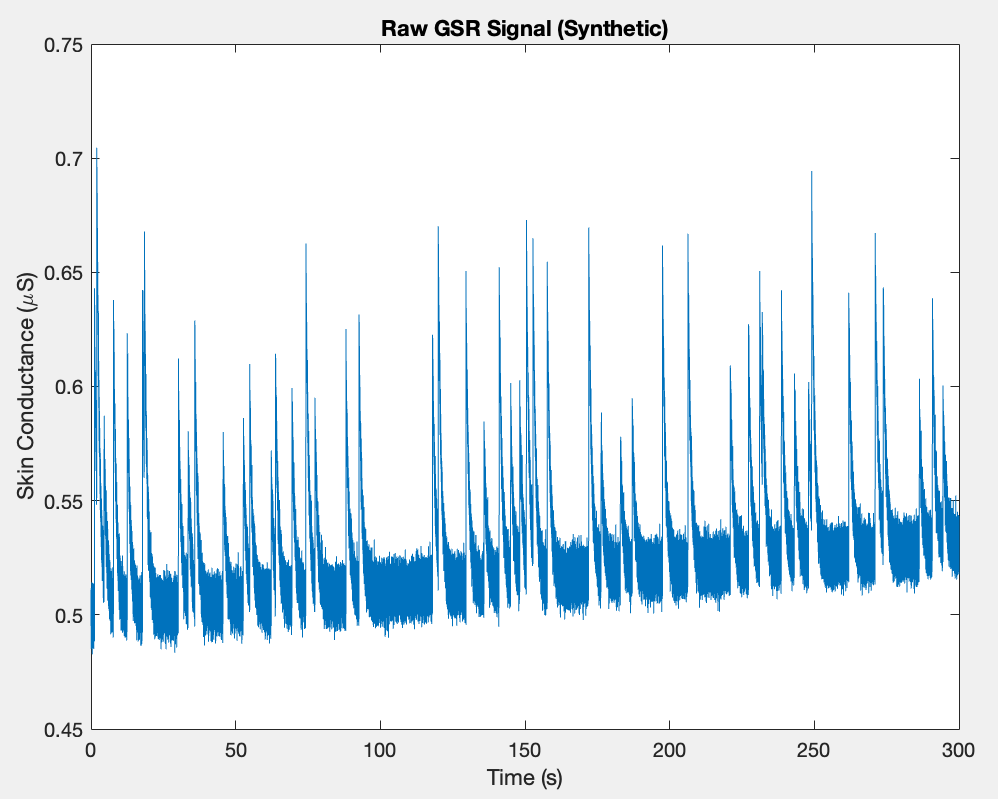
\includegraphics[width=\linewidth]{figure_1.png}
\caption{Raw GSR Signal (Synthetic)}
\label{fig:raw_gsr_signal}
\end{figure}

\paragraph{Description}

Figure \ref{fig:raw_gsr_signal} displays the synthetic GSR signal generated by combining the tonic and phasic components with added Gaussian noise. The tonic component manifests as a slow upward trend, representing the baseline skin conductance level that gradually drifts over time. The phasic component consists of sharp, transient peaks corresponding to simulated Skin Conductance Responses (SCRs) occurring at random times.

\paragraph{Interpretation}

The raw GSR signal demonstrates the typical features of a physiological GSR recording, including both slow baseline fluctuations and rapid responses to stimuli. The presence of noise mimics real-world measurement conditions, making the synthetic signal a suitable candidate for testing the preprocessing and decomposition methods.

\subsection*{Figure 2: Preprocessed GSR Signal}

\begin{figure}[H]
\centering
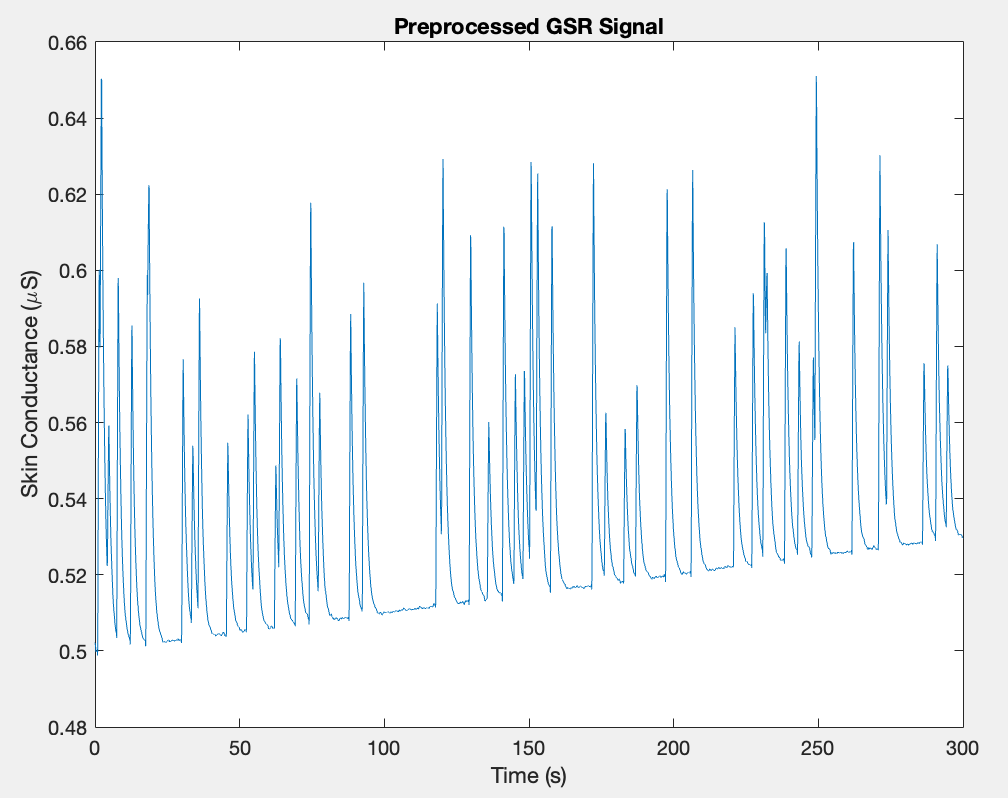
\includegraphics[width=\linewidth]{figure_2.png}
\caption{Preprocessed GSR Signal}
\label{fig:preprocessed_gsr_signal}
\end{figure}

\paragraph{Description}

Figure \ref{fig:preprocessed_gsr_signal} shows the GSR signal after applying preprocessing steps, including low-pass filtering, downsampling, and smoothing. The high-frequency noise present in the raw signal has been significantly reduced, and the essential features of the tonic and phasic components are preserved.

\paragraph{Interpretation}

The preprocessing enhances the signal quality by removing unwanted noise and reducing data size without losing critical information. This step is crucial for accurate decomposition, as it ensures that the subsequent analysis operates on a clean and representative signal.

\subsection*{Figure 3: Impulse Response Function (IRF)}

\begin{figure}[H]
\centering
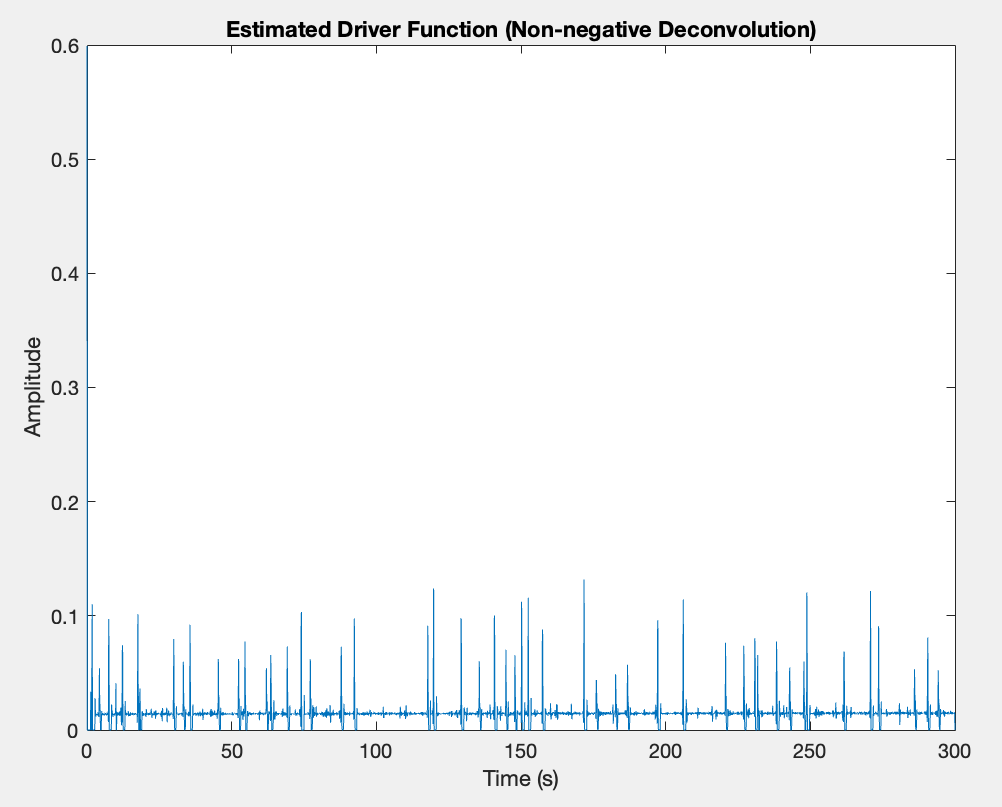
\includegraphics[width=\linewidth]{figure_3.png}
\caption{Impulse Response Function (IRF)}
\label{fig:irf}
\end{figure}

\paragraph{Description}

Figure \ref{fig:irf} depicts the Impulse Response Function (IRF) used in the deconvolution process. The IRF is a biexponential function modeling the skin conductance response to a unit neural impulse, characterized by a rapid rise and a slower decay.

\paragraph{Interpretation}

The IRF captures the typical dynamics of an SCR, with parameters $\tau_1$ and $\tau_2$ representing the rise and decay time constants, respectively. It serves as a mathematical representation of how neural activations translate into observable changes in skin conductance.

\subsection*{Figure 4: Estimated Driver Function}

\begin{figure}[H]
\centering
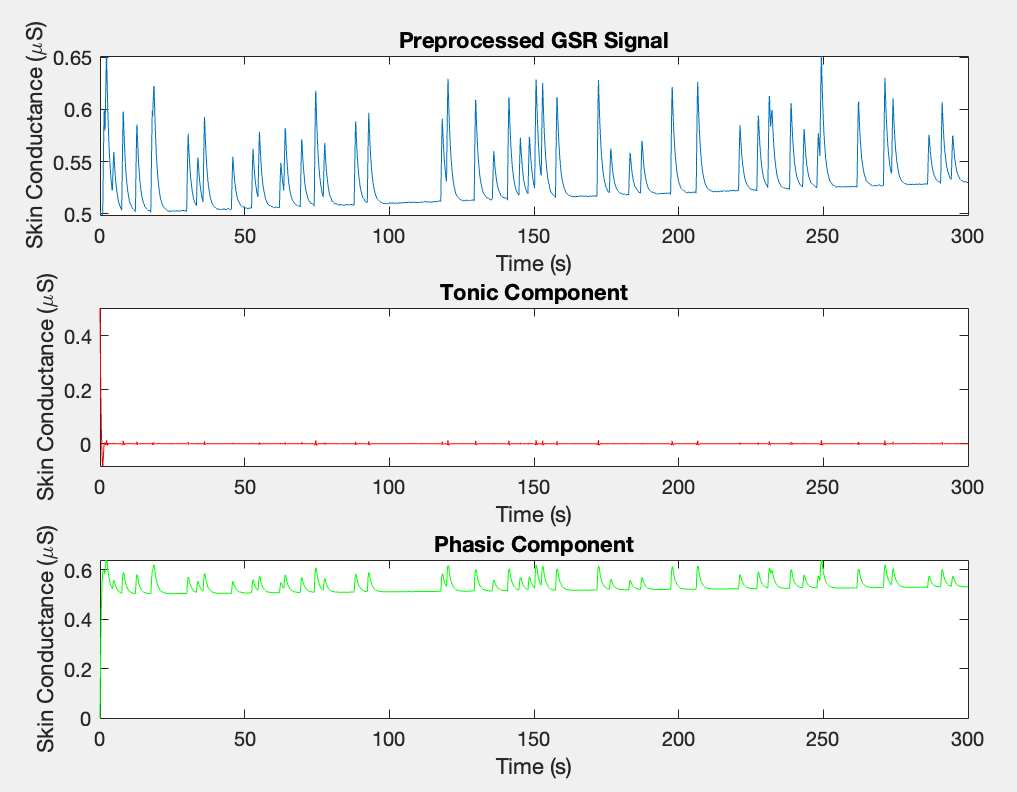
\includegraphics[width=\linewidth]{figure_4.png}
\caption{Estimated Driver Function (Non-negative Deconvolution)}
\label{fig:driver_function}
\end{figure}

\paragraph{Description}

Figure \ref{fig:driver_function} presents the estimated driver function obtained through non-negative deconvolution of the preprocessed GSR signal. The driver function reveals the underlying neural activations responsible for generating the phasic component of the GSR signal.


\paragraph{Interpretation}

The peaks in the driver function correspond to the estimated timings of sympathetic nervous system activations. The non-negativity constraint ensures that the driver function represents physiologically plausible neural activity. This function provides valuable insights into the temporal patterns of neural responses.

\subsection*{Figure 5: Decomposed GSR Components}

\begin{figure}[H]
\centering
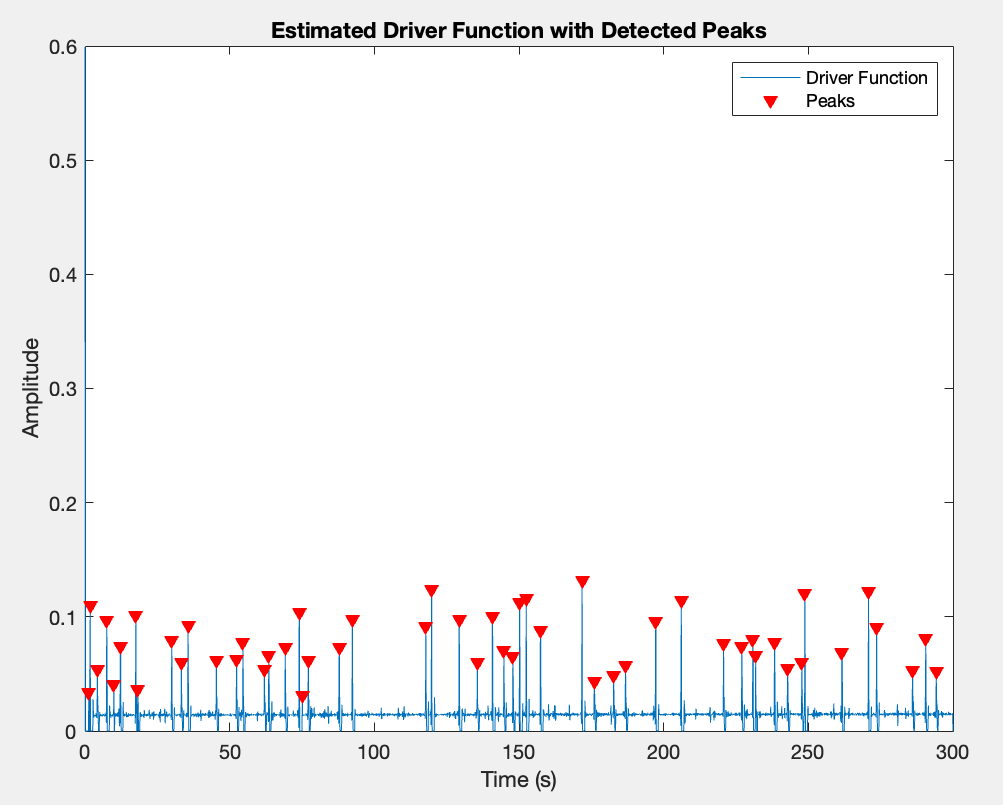
\includegraphics[width=\linewidth]{figure_5.png}
\caption{Decomposed GSR Components}
\label{fig:decomposed_components}
\end{figure}

\paragraph{Description}

Figure \ref{fig:decomposed_components} displays the decomposition of the preprocessed GSR signal into its tonic and phasic components. The figure consists of three subplots:

\begin{enumerate}
    \item \textbf{Preprocessed GSR Signal}: The original signal after preprocessing.
    \item \textbf{Tonic Component}: The slow-varying baseline conductance level.
    \item \textbf{Phasic Component}: The rapid fluctuations due to SCRs.
\end{enumerate}

\paragraph{Interpretation}

The decomposition illustrates how the phasic component captures the transient responses associated with neural activations, while the tonic component reflects the underlying baseline conductance. By separating these components, researchers can analyze the phasic activity independently, facilitating a more focused examination of sympathetic nervous system responses.

\section*{Conclusion}

Continuous Decomposition Analysis provides a powerful framework for dissecting GSR signals into their constituent components. By applying non-negative deconvolution techniques to the preprocessed GSR data, it is possible to estimate the underlying neural driver function and reconstruct the phasic and tonic components. This approach enhances the interpretability of GSR signals and facilitates more accurate psychophysiological analyses.

Understanding the mathematical foundations of CDA and the preprocessing steps involved is crucial for researchers working with GSR data. Proper implementation of these methods enables the extraction of meaningful physiological information.

\bibliography{citations}

\end{document}